\documentclass[
	12pt,				% tamanho da fonte
	oneside,			% para impressão em recto e verso. Oposto a oneside
	a4paper,			% tamanho do papel. 
	english,			% idioma adicional para hifenização
	brazil,				% o último idioma é o principal do documento
	]{abntex2}

% ---
% Pacotes fundamentais 
% ---
\usepackage{lmodern}			% Usa a fonte Latin Modern
\usepackage[T1]{fontenc}		% Selecao de codigos de fonte.
\usepackage[utf8]{inputenc}		% Codificacao do documento (conversão automática dos acentos)
\usepackage{indentfirst}		% Indenta o primeiro parágrafo de cada seção.
\usepackage{color}				% Controle das cores
\usepackage{graphicx}			% Inclusão de gráficos
\usepackage{microtype} 			% para melhorias de justificação
\usepackage{multicol}
\usepackage{multirow}
\usepackage[brazilian,hyperpageref]{backref}	 % Paginas com as citações na bibl
\usepackage[alf]{abntex2cite}	% Citações padrão ABNT
\usepackage{float}
% --- 
% CONFIGURAÇÕES DE PACOTES
% --- 

% ---
% Configurações do pacote backref
% Usado sem a opção hyperpageref de backref
\renewcommand{\backrefpagesname}{Citado na(s) página(s):~}
% Texto padrão antes do número das páginas
\renewcommand{\backref}{}
% Define os textos da citação
\renewcommand*{\backrefalt}[4]{
	\ifcase #1 %
		Nenhuma citação no texto.%
	\or
		Citado na página #2.%
	\else
		Citado #1 vezes nas páginas #2.%
	\fi}%
% ---

% ---
% Informações de dados para CAPA e FOLHA DE ROSTO
% ---
    \titulo{Prática 18: Computação Evolucionária - Crossover}
\autor{Pedro Inácio Rodrigues Pontes}
\local{Belo Horizonte, Brasil}
\data{2024}
\instituicao{%
  Universidade Federal de Minas Gerais
  \par
  Colégio Técnico
  \par
  Curso Técnico em Desenvolvimento de Sistemas}

\definecolor{blue}{RGB}{41,5,195}

\makeatletter
\hypersetup{
     	%pagebackref=true,
		pdftitle={\@title}, 
		pdfauthor={\@author},
    	pdfsubject={\imprimirpreambulo},
		colorlinks=true,       		% false: boxed links; true: colored links
    	linkcolor=blue,          	% color of internal links
    	citecolor=blue,        		% color of links to bibliography
    	filecolor=magenta,      		% color of file links
		urlcolor=blue,
		bookmarksdepth=4
}
\makeatother

\renewcommand{\thesection}{\arabic{section}}
\setlength{\parindent}{1.3cm}
\setlength{\parskip}{0.2cm} 

\makeindex


\begin{document}

\selectlanguage{brazil}
\frenchspacing 

\imprimircapa

{
\ABNTEXchapterfont

\textual

% ----------------------------------------------------------
% Introdução (exemplo de capítulo sem numeração, mas presente no Sumário)
% ----------------------------------------------------------
\section{Introdução}

O objetivo da atividade é implementar o processo de reprodução sexuada e crossover nos organismos criados no programa previamente fornecido que simula uma rede de organismos com diversar gerações e características que são repassadas pelo DNA. O crossover foi ditado para ter 50\% do DNA da mãe e 50\% do DNA do pai.

\subsection{Objetivos}

\textbf{Práticos}
\begin{itemize}
\item Adicionar um atributo sexo para cada organismo.
\item Criar um mecanismo para ditar quando os organismos irão se reproduzir com base no conceito de reprodução sexuada.
\item Criar uma maneira de fazer o crossover do DNA
\end{itemize}

\textbf{Teóricos}
\begin{itemize}
    \item Desenvolver o conceito de programação evolucionária/voltada a replicar o mundo real.
\end{itemize}
\section{Desenvolvimento}

\subsection{Resolução do Atributo Sexo para cada Organismo}

Criado o atributo \textit{int sexo}, o qual armazena 0 para machos e 1 para fêmeas.

Para definir o sexo, foi utilizada uma solução arbitrária, que consiste em atribuir 0 quando a soma dos atributos tamanho, percepção e velocidade é par, e 1 quando é impar:

\begin{itshape}
this.sexo = ((int)(this.velocidadeMax + this.tamanho + this.percepcao) \% 2) == 0 ? 0 : 1; 
\end{itshape}

\subsection{Resolução da Implementação da Reprodução Sexuada}

Criada a função \textit{temSexoDiferente}, a qual retorna o que é proposto em seu nome. Compara o objeto em questão com outro fornecido nos parâmetros da função.

Criada a função procura parceiro, a qual itera sobre toda a população e só para após encontrar outro organismo a menos de 50 pixels de distância do organismo analisado e que possui sexo diferente. Retorna o organismo encontrado.

\begin{verbatim}
  Organismo procuraParceiro() {
    Organismo maisProximo = null;

    for (Organismo r : populacao) {
      float d = PVector.dist(posicao, r.posicao);
      if (d < 50 && temSexoDiferente(r)) {
        maisProximo = r;
        break;
      }
    }
    return maisProximo;
 }
\end{verbatim}

\subsubsection{Resolução do Crossover}

Adicionado um for dentro de reproduzir que, com uma chance de 50\%, dá ou o DNA da mãe ou do pai para um pedaço de DNA do filho. O for itera sobre as 3 partes do DNA.

\begin{verbatim}
     for (int i = 0; i < dna.length; i++) {
          if (floor(random(0,2)) == 0){
            novoDna[i] = dna[i];
          }
          else{
            novoDna[i] = parceiro.dna[i];
          }
      }
\end{verbatim}
\subsection{Extra}

É desenhada uma elipse temporária de cor preta num raio de 100 pixels de onde ocorreu a reprodução sexuada e nasceu um novo organismo.

\section{Resultados}

\begin{figure}[H]
\centering
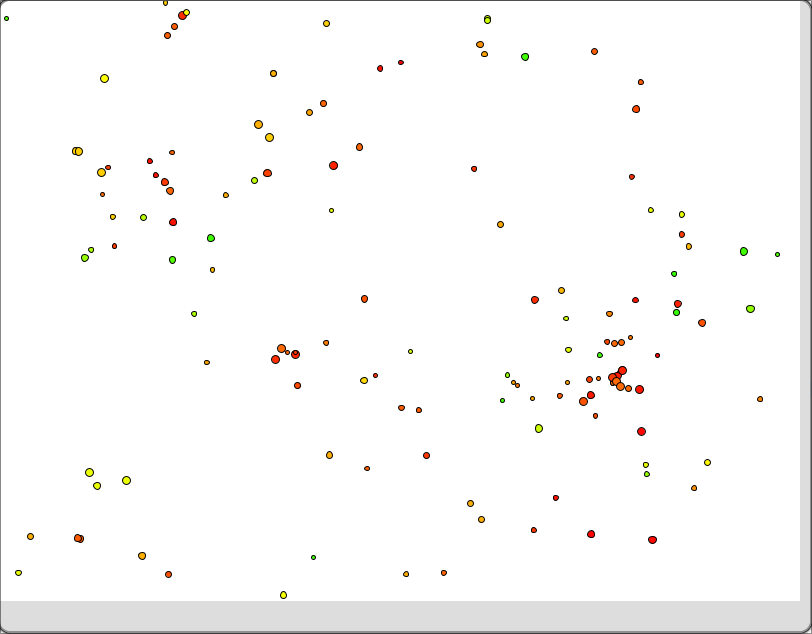
\includegraphics[width=0.9\textwidth]{imgs/img1.png}
\caption{Colônia de organismos em estado neutro}
\label{imagem 1}
\end{figure}
\begin{figure}[H]
\centering
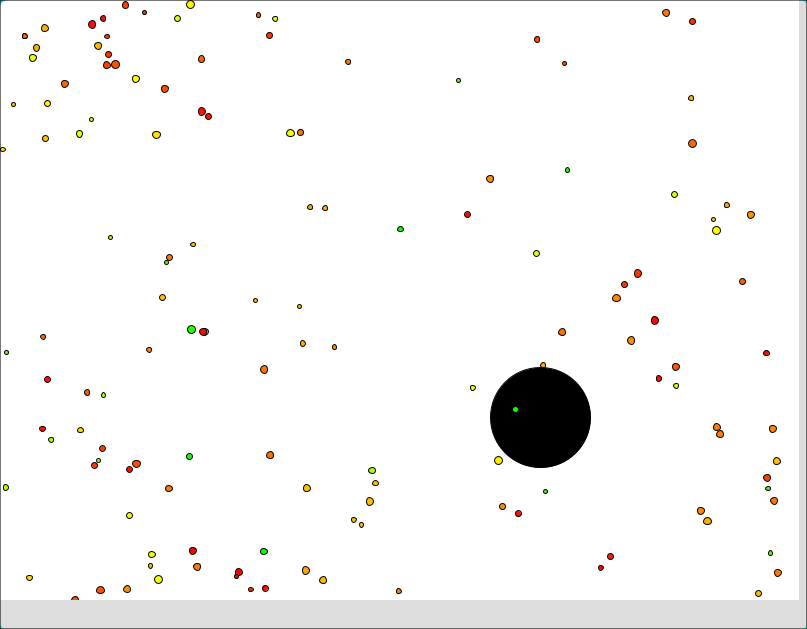
\includegraphics[width=0.9\textwidth]{imgs/img2.png}
\caption{Colônia de organismos após a ocorrência da reprodução sexuada}
\label{imagem 2}
\end{figure}

Os resultados dessa prática são extremamente abstratos, mas conseguem ser observados pela ocorrência das rápidas elipses negras sempre que ocorre a reprodução sexuada e pela diminuição ou aumento exponencial da população conforme a definição da distância mínima para reprodução sexuada. O crossover é difícil de ser idêntificado, sendo mais palpável apenas dentro das linhas de código, mas é visto quando os organismos possuem algumas características semelhantes ou análogas de velocidade, percepção e tamanho, pois o DNA dos pais que é herdado.

\section{Conclusão}

Os resultados encontrados foram de acordo com o esperado. A prática permitiu o melhor entendimento de como replicar situações reais no mundo computacional e simular ambientes. Uma melhoria ao código poderia ser a implementação de alguma funcionalidade que permitisse a visibilidade de características originadas e passadas pela implementação do crossover.

\end{document}
